%!TEX program = xelatex



\documentclass[cn,black,10pt,normal]{elegantnote}
\usepackage{float}
\usepackage{hyperref}


%\newcommand{\upcite}[1]{\textsuperscript{\textsuperscript{\cite{#1}}}}

\title{数码摄影作业(10)后期曲线}
\author{姓名:姜文渊\\学号:1951510}
%\institute{School of Life Science, Tongji University}
%\version{1.00}
\date{2021年5月9日}

\begin{document}

\maketitle

\section{调整前的图片}

\begin{figure}[H]
    \centering
    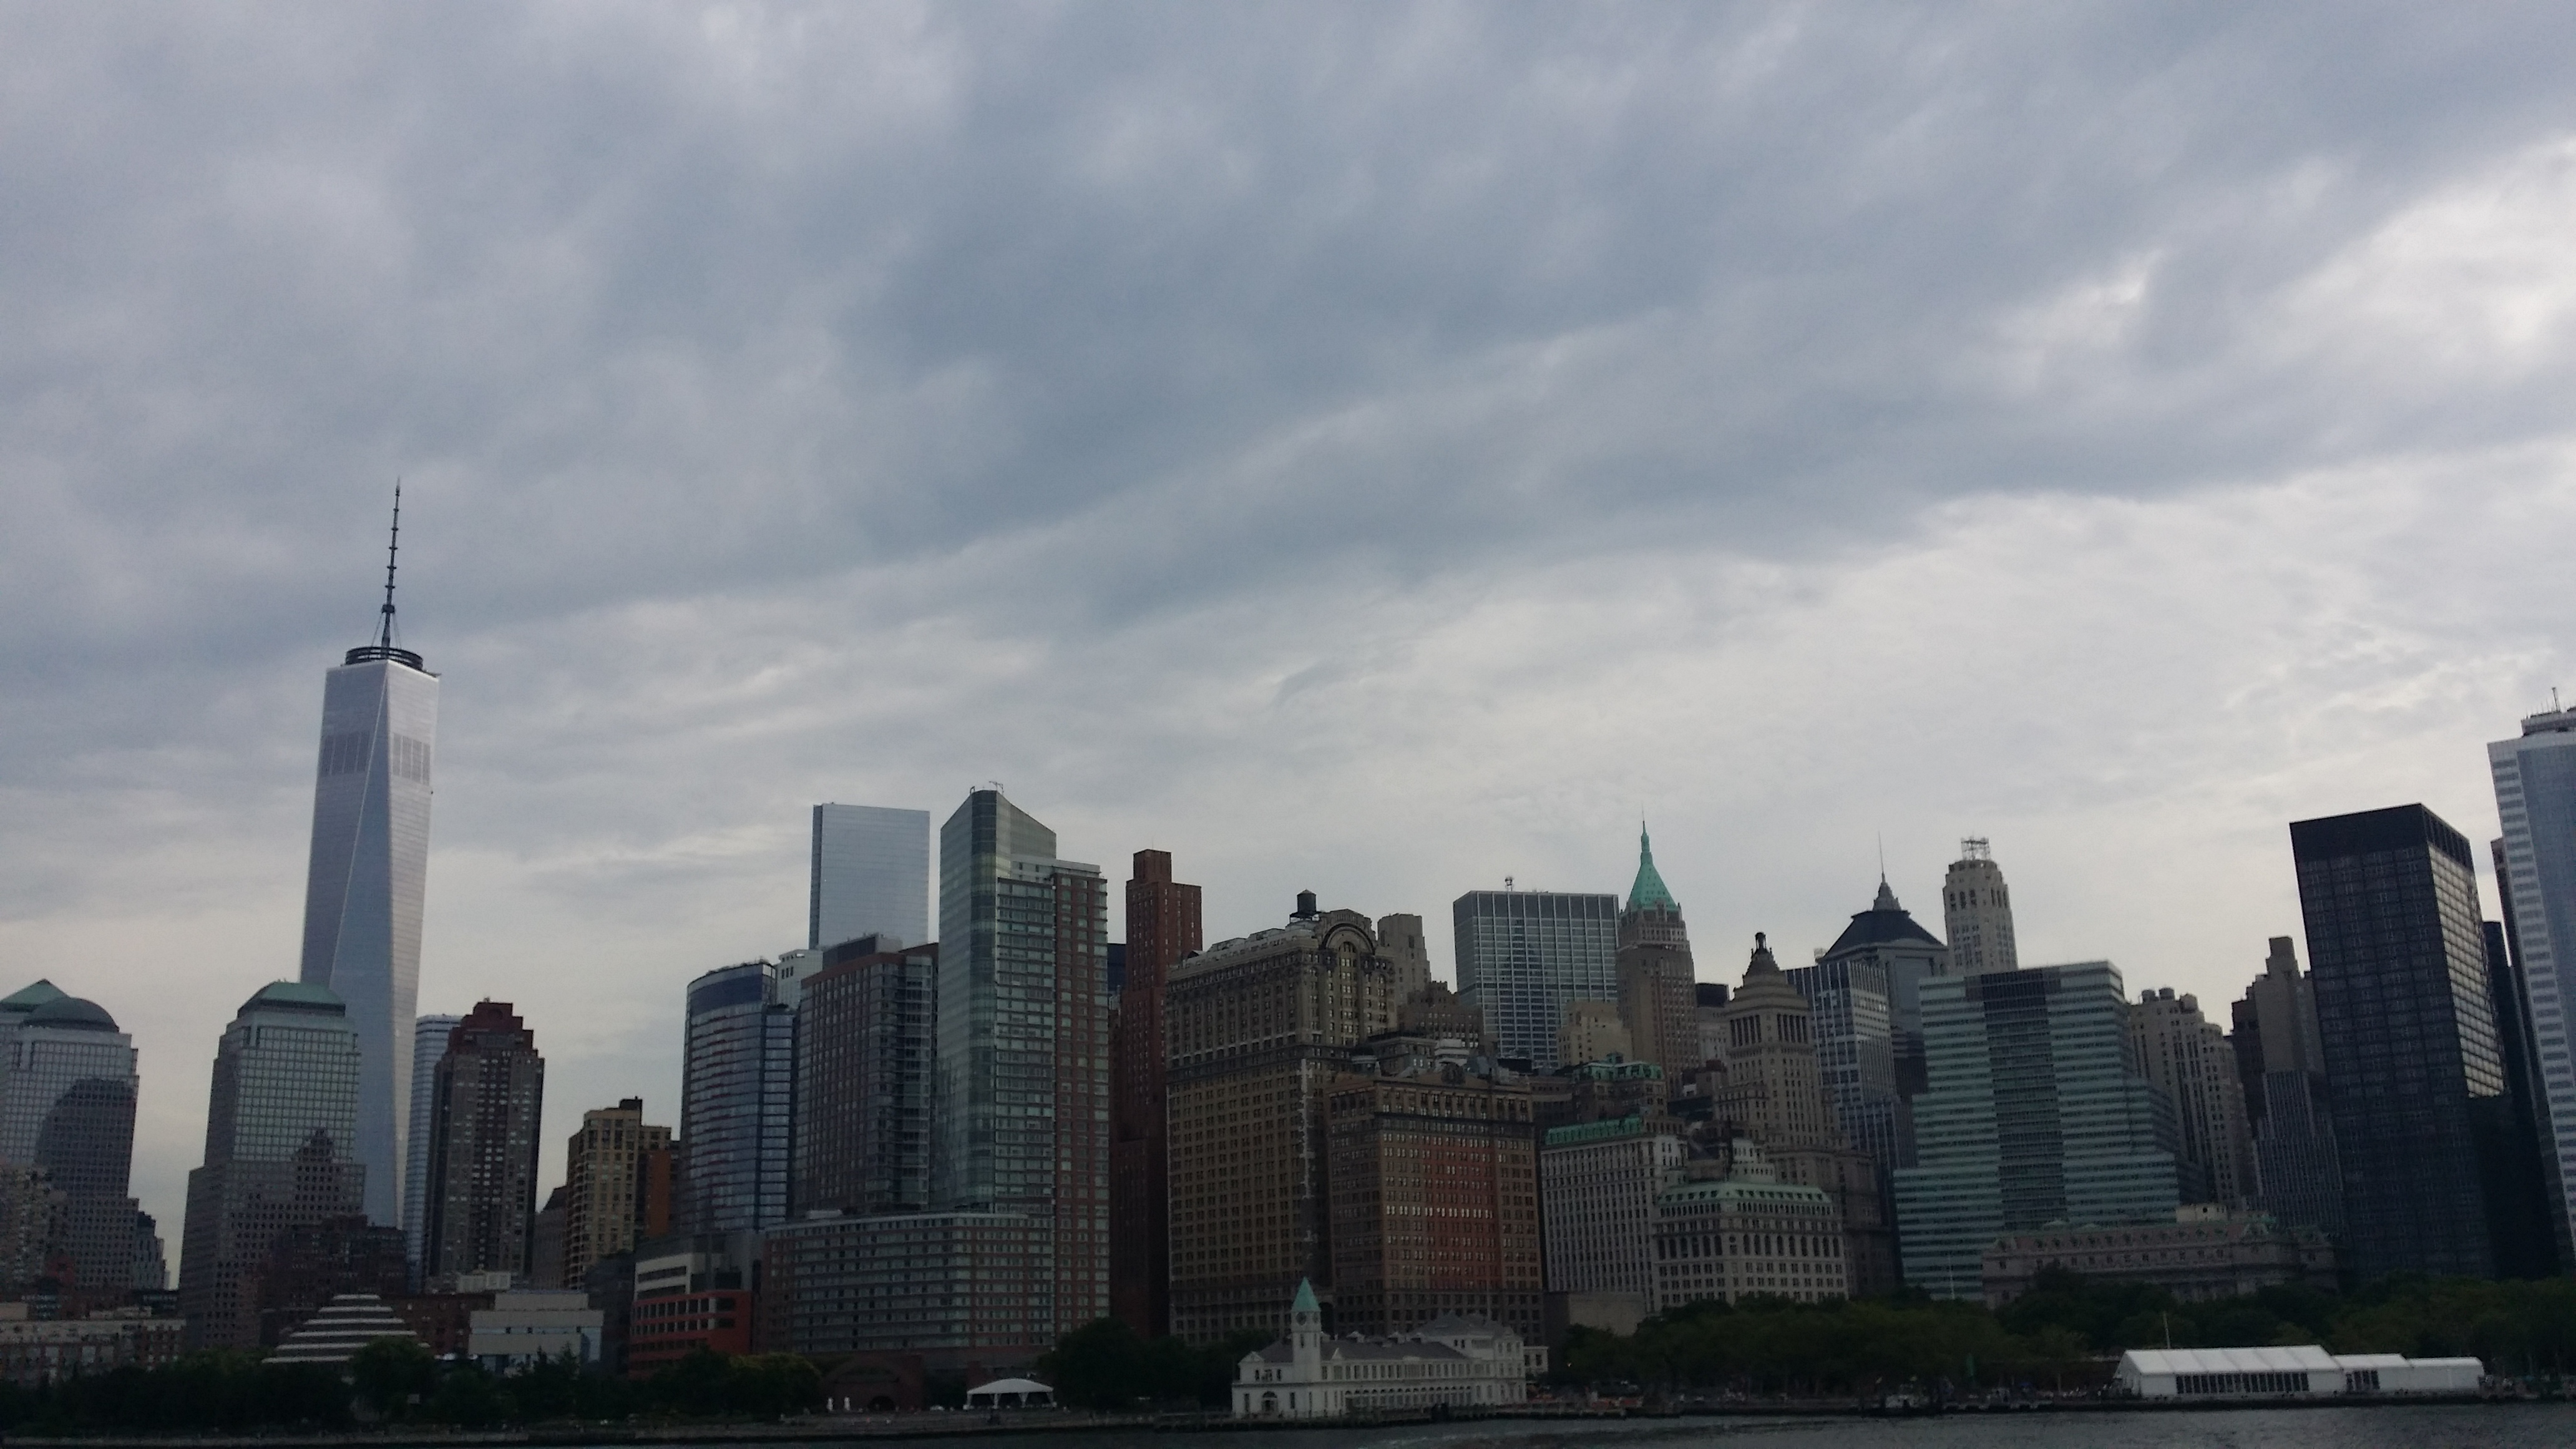
\includegraphics[width=0.5\textwidth]{F1}
    %\caption{From “Pacific Theater,” WWII, 1942-45 \\ 路易斯·蒙巴顿勋爵上将在萨拉托加号上向人员致辞}
    \label{F-02}
\end{figure}

该图片拍摄与学校篮球场附近,时天色已晚,图像色调较暗,且树叶之间的颜色对比不明显。

\section{调整后的图片}

\begin{figure}[H]
    \centering
    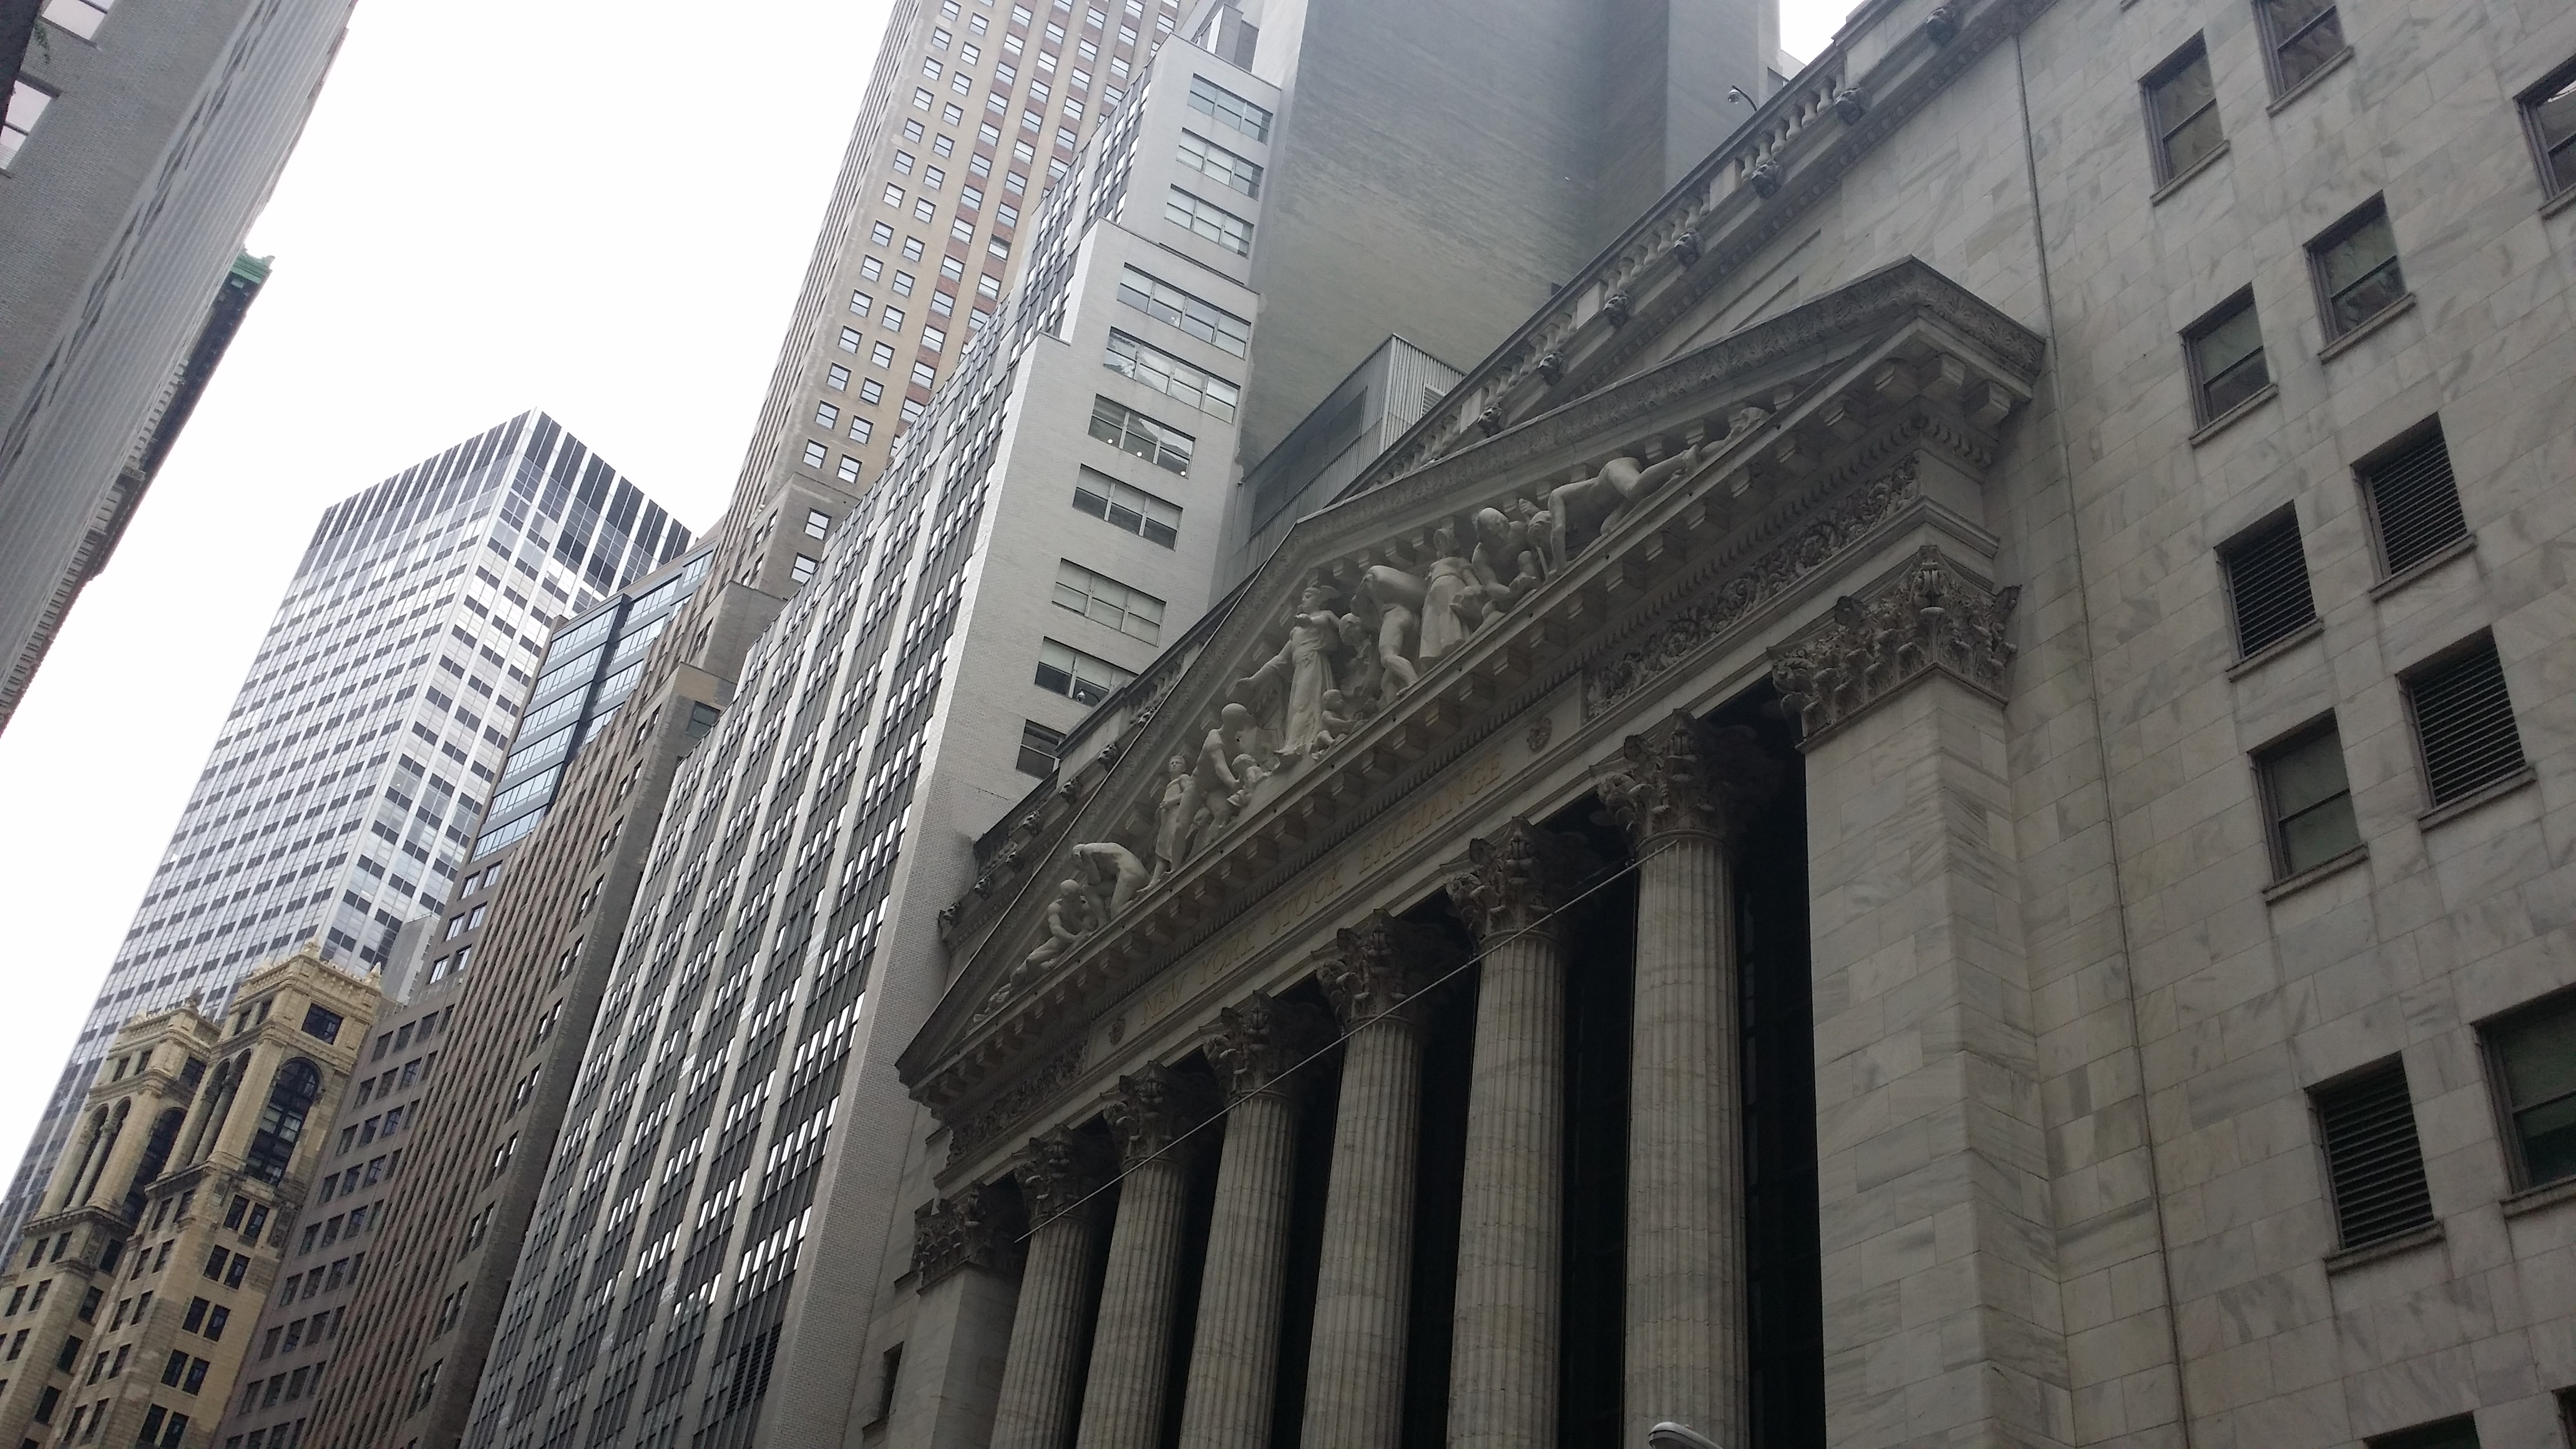
\includegraphics[width=0.5\textwidth,angle=0]{F2}
    %\caption{From “Pacific Theater,” WWII, 1942-45 \\ 士兵受伤流血的手}
    \label{F-01}
\end{figure}

经掐头去尾,中间将曲线调整为上凸的形状后,对比度有所好转,可见照片中树叶分红绿两色。


%\bibstyle{unsrt}
%\bibliography{references}{}
\end{document}
